\documentclass[11pt, a4paper, table]{article}
\usepackage[dvipsnames]{xcolor}
\usepackage{tikz}
\usepackage{amsmath}
\usepackage{amsthm}
\usepackage[dutch]{babel}
\usepackage[latin1]{inputenc} 
\usepackage{float}
\usepackage{algpseudocode}
\usepackage{algorithm}
\usepackage{textcomp}
\usepackage{rotating}
\usepackage[section]{placeins}
\usepackage[skins]{tcolorbox}
\usepackage{csvsimple}

\makeatletter
\newenvironment{algoritme}[1][H]{%
	\renewcommand{\ALG@name}{Algoritme}% Update algorithm name
	\renewcommand{\algorithmicrequire}{\textbf{Input:}}
	\renewcommand{\algorithmicensure}{\textbf{Output:}}
	\begin{algorithm}[#1]%
	}{\end{algorithm}}
\makeatother
\setlength{\parindent}{0pt}

\theoremstyle{definition}
\newtheorem{opgave}{Opgave}
\theoremstyle{definition}
\newtheorem{definitie}{Definitie}
\theoremstyle{definition}
\newtheorem{opmerking}{Opmerking}
\newtheorem{stelling}{Stelling}
\newtheorem{lemma}{Lemma}


\begin{document}
	\title{Project Gretige Algoritmen}
	\author{Jarre Knockaert}
	\maketitle
	
\thispagestyle{empty}
\newpage
\pagenumbering{arabic}

\section{Definities}
Eerst bespreek ik enkele termen die ik in het verslag zal gebruiken.
\begin{definitie}
	Een \textbf{dominante verzameling} van een graaf G is een deelverzameling D(G) van V(G) zodat elke top uit V(G) ofwel element is van D(G) ofwel adjecent is met een top uit D(G). 
	\begin{equation}
	D(G) = \{v \in V(G) \mid v \in D(G) \vee (w \in D(G) \land vw \in E(G)\}
	\end{equation}
\end{definitie}
\begin{definitie}
	Een top v wordt gemarkeerd met \textbf{bezocht} als v element is van de dominante verzameling.
\end{definitie}
\begin{definitie}
	Een top v is een \textbf{buur} van een top w als de toppen adjecent zijn, m.a.w. $v \in N_G(w)$
\end{definitie}
\begin{definitie}
	De \textbf{coverage} of \textbf{bedekking} van een top v stelt een bovengrens voor van de bijdrage van top aan de dominante verzameling. Deze bijdrage is het maximale aantal toppen die toegevoegd worden aan de dominante lijst door het toevoegen van v aan D(G). 
	\begin{equation}
	coverage(v) \geq \vert \{w \in V(G) \mid w \in \{v \cup N_G(v)\} \land w \not\in D(G) \}\vert
	\end{equation}
\end{definitie}
\begin{definitie}
	De \textbf{actual coverage} of \textbf{werkelijke bedekking} van een top v stelt de eigenlijke bijdrage van v voor aan de dominante verzameling. Deze bijdrage is het exacte aantal toppen die toegevoegd worden aan de dominante lijst door het toevoegen van v aan D(G).
	\begin{equation}
	actualCoverage(v) = \vert \{w \in V(G) \mid w \in \{v \cup N_G(v)\} \land w \not\in D(G) \}\vert
	\end{equation} 
\end{definitie}
\begin{opmerking}
	De werkelijke coverage of werkelijke bedekking van een verzameling is de
	som van van de werkelijke coverage of werkelijke bedekking van elke top uit die verzameling. Hierbij moet rekening gehouden worden dat door het toevoegen van de ene top aan de dominante verzameling, de werkelijke bedekking kan wijzigen van de andere top. Met andere woorden is het dus het aantal toegevoegde elementen aan de dominante verzameling na het toevoegen van elke top uit de verzameling. 
\end{opmerking}
\begin{definitie}
	Twee bogen (e,e') zijn een \textbf{paar} als ze \'{e}\'{e}n gemeenschappelijke top delen. Elk paar met de bogen e, e' maakt deel uit van juist \'{e}\'{e}n vlak $f_G(e,e')$. 
\end{definitie}
\begin{opmerking}
	Het midden of het centrum van een paar met de bogen e, e'  gemeenschappelijke top van twee verbonden bogen. De eindpunten zijn de overige twee toppen van dit paar. De vlakken waartoe een top v behoort, zijn de vlakken van de paren waarvan v het centrum is. De paren van een vlak V zijn alle paren zodat $f_G(e,e')=V$.
\end{opmerking}
\begin{opmerking}
	Twee vlakken zijn aanliggend als deze vlakken \'{e}\'{e}n boog gemeenschappelijk hebben. Deze vlakken zijn buren. 
\end{opmerking}
\begin{definitie}
	De twee toppenverzamelingen $D_1$ en $D_2$ van een graaf zijn \textbf{onafhankelijk} als en slechts $D_1 \cap D_2 = \emptyset$
\end{definitie}
\section{Theoretische vragen}
\begin{opgave}
	Indien er 2 naburige toppen v en w een grote bedekking leveren, zal de top v met de hoogste graad worden toegevoegd aan de dominante verzameling en de buren zullen worden verwijderd. Het zou echter beter zijn om zowel v en w toe te voegen aan de dominante verzameling, want w zorgt ook voor een hoge toename van de bedekking van de dominante verzameling. 
	Een voorbeeld van dergelijk geval, een graaf waarbij het algoritme zeer slecht presteert, zie je op figuur \ref{fig:worstcase}. Als we het algoritme uitvoeren op de graaf gebeurt het volgende:
	\begin{itemize}
		\item Neem top v = $4k+1$ met hoogste graad: $2k-1$. (Dit kon evengoed top $4k+2$ zijn, aangezien zijn graad gelijk is.)
		\item Voeg v toe aan de dominante lijst D. 
		\item Verwijder v en al zijn buren (top $1$ tot en met top $2k$) uit de graaf G. Nu bevat de G nog $2k-1$ toppen (top $2k+1$ tot en met top $4k$).
		\item De resterende toppen uit de graaf hebben elk graad 0 en zijn ge\"{i}soleerde toppen. (Aangezien hun enige buur werd verwijderd uit de graaf.) Voor elke top w van $2k+1$ tot en met top $4k$ gebeurt nu het volgende:
		\begin{itemize}
			\item Neem de top w. Aangezien elke top graad 0 heeft maakt het niet uit welke top we uit de graaf kiezen. Hun graad is (en blijft) gelijk aan elkaar. 
			\item Voeg w toe aan D. 
			\item Verwijder w uit G. De top w is ge\"{i}soleerd en dus er zullen ook geen extra toppen uit de graaf verwijderd worden. 
		\end{itemize}
	\end{itemize}
	In totaal werden $2k$ toppen toegevoegd aan de dominante lijst: top $4k+1$ en top $2k+1$ tot en met top $4k$. De minimale dominante verzameling bevat echter enkel de 2 toppen $4k+1$ en $4k+2$. 
	Het resultaat van het algoritme is een dominante verzameling met $\frac{2k}{2}=k$ keer meer toppen meer dan de optimale dominante verzameling. 
	\begin{figure}[H]
	%\centering
		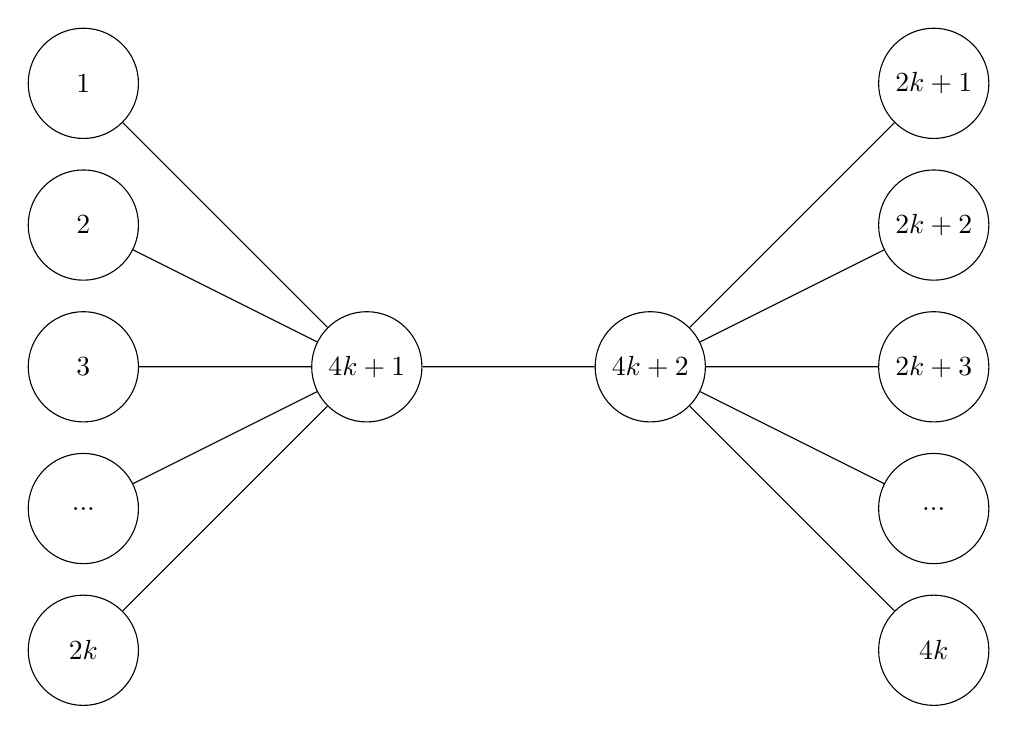
\begin{tikzpicture} 
		[main node/.style={circle, draw, minimum width=1.4cm, minimum height=1.4cm}, scale=1.8]
		\def\length{3}
			\foreach \a in {1,2,...,\length}{
				\node[main node]  (\a) at (0, 2+\length-\a) {$\a$};
				\node[main node]  (2k+\a) at (6, 2+\length-\a) {$2k+\a$};
			}
			\node[main node]  (leftdots) at (0, 1) {...};
			\node[main node]  (rightdots) at (6, 1) {...};
			\node[main node]  (2k) at (0, 0) {$2k$};
			\node[main node]  (4k) at (6, 0) {$4k$};
			\node[main node] (4k+1) at (2,2) {$4k+1$}; 
			\node[main node] (4k+2) at (4,2) {$4k+2$}; 
	
			\path (leftdots) edge node {} (4k+1);
			\path (rightdots) edge node {} (4k+2);
			\path (4k+1) edge node {} (4k+2);
			\path (2k) edge node {} (4k+1);
			\path (4k) edge node {} (4k+2);
			\foreach \a in {1,2,...,\length}{
				\path (\a) edge node {} (4k+1);
				\path (2k+\a) edge node {} (4k+2);
			}
		\end{tikzpicture}
		\caption{Een graaf waarbij het algoritme slecht presteert.}
		\label{fig:worstcase}
	\end{figure}
\end{opgave}
\begin{opgave}
	Beschouw de duale graaf DG(V(DG), E(DG)) verkregen door de vlakke triangulatie G. 
	\begin{stelling}
		\label{stelling1}
		Voor een vlakke triangulatie liggen er binnen en buiten de hamiltoniaanse cykel evenveel vlakken. 
	\end{stelling}
	Merk eerst op dat de ge\"{i}nduceerde deelgrafen samenhangend moeten zijn aangezien de vlakken vermeld in stelling \ref{stelling1} gescheiden zijn door een hamiltoniaanse cykel. Alle vlakken uit \'{e}\'{e}n vlakkenverzameling moeten dus samen ofwel binnen ofwel buiten de cykel liggen. 
	\begin{opmerking}
		\label{opmerking1}
		Alle toppen op de gemeenschappelijke bogen van vlakken uit de twee verschillende vlakkenverzamelingen zullen deel uitmaken van de hamiltoniaanse cykel. 
	\end{opmerking}
	De reden hiervoor is eenvoudig, aangezien er juist 2 vlakkenverzamelingen zijn, en alle vlakken van een vlakkenverzameling ofwel binnen ofwel buiten de cykel ligt, wordt de cykel gedefinieerd door elk gemeenschappelijk boog van alle paren van vlakken zodat de beide vlakken tot een verschillende vlakkenverzameling behoren. Voor het bewijs van stelling \ref{stelling1} hebben we eerst volgende lemma's nodig. 

	\begin{lemma}	
		\label{lemma1}
		Beschouw een vlakke	triangulatie G en zijn duale graaf DG. 
		Beschouw verder de ge\"{i}nduceerde deelgrafen van de twee onafhankelijke toppenverzamelingen $D_1$ en $D_2$ zodat $D_1, D_2 \in V(DG) , D_1 \cup D_2 = V(DG)$.  Als $D_1$ en $D_2$ de vlakken resp. binnen en buiten de hamiltoniaanse cykel voorstellen, dan zijn $DG_1$ en $DG_2$ een boom.   
		
	\end{lemma}
	
	\begin{proof}
		Beschouw twee onafhankelijke toppenverzamelingen $D_1$ en $D_2$ in de duale graaf DG van de vlakke triangulatie G zodat $D_1 \cup D_2 = V(DG)$. Stel dat eender van de toppenverzamelingen $D_1$ een deelgraaf met \'{e}\'{e}n cykel induceert. Aangezien de duale graaf een 3-reguliere graaf is, moet elke top uit de cykel minstens 2 buren hebben in de gekozen toppenverzameling. Als dit niet zo is, vormen de toppen geen cykel. Beschouw nu de ge\"{i}nduceerde deelgrafen $DG_1$ en $DG_2$ van respectievelijk $D_1$ en $D_2$. De deelgraaf $DG_2$ (en dus $D_2$) moet volledig binnen ofwel volledig buiten de cykel liggen aangezien de toppenverzamelingen samenhangend moeten zijn. 
		\\\\Stel eerst dat $DG_2$ binnenin de cykel ligt. Neem de vlakkenverzamelingen $V_1$ en $V_2$ van de vlakke triangulatie G  gegeven door resp. de toppen van $D_1$ en $D_2$. E\'{e}n of meerdere vlakken in G verkregen met de toppen van de cykel van $DG_1$ zullen een gemeenschappelijke boog hebben met een vlak uit $V_2$. Dergelijk vlak uit $V_1$ heeft dus twee buren in $V_1$ en 1 buur in $V_2$, wat betekent dat beide vlakken juist twee toppen gemeenschappelijk hebben. De overige derde top uit de vlakke triangulatie maakt echter deel uit van de twee gemeenschappelijke bogen met de vlakken uit de cykel van $DG_1$.  Nu wegens opmerking \ref{opmerking1} geldt dat deze top niet deel uitmaakt van de cykel van de vlakke triangulatie, zodat de cykel in dit geval geen hamiltoniaanse cykel is.
		\\\\Stel vervolgens dat $DG_2$ buiten de cykel ligt. Elk vlak heeft opnieuw 2 bogen gemeenschappelijk met aanliggende vlakken uit de cykel. Deze bogen zullen aan \'{e}\'{e}n eindpunt t snijden, het andere eindpunt van beide bogen zullen opnieuw een boog vormen. Deze boog is een een gemeenschappelijk boog met een vlak buiten de cykel. Aangezien er binnenin de cykel geen vlakken liggen van $DG_2$, zal t nooit deel uitmaken van een boog van $DG_2$, en zal dus geen deel uitmaken van een gemeenschappelijk boog van 2 vlakken uit een verschillende vlakkenverzameling. Vanwege opmerking \ref{opmerking1} geldt dat deze top niet deel uitmaakt van de cykel van de vlakke triangulatie, zodat de cykel in dit geval geen hamiltoniaanse cykel is. 
		\\\\Aangezien enkel vorige twee gevallen mogelijk zijn (zoals besproken voor de individuele bespreking van de gevallen), zal er altijd minstens \'{e}\'{e}n top geen deel uitmaken van de cykel van de vlakke triangulatie, waardoor de cykel geen hamiltoniaanse cykel is. Hieruit kunnen we besluiten dat de deelgrafen $DG_1$ en $DG_2$ geen cykel mogen bevatten en dus een boom moeten zijn.
	\end{proof}
	Volgend lemma en zijn bewijs werd ge\"{i}nspireerd door het artikel "To be or not to be Yutsis". 
	\begin{lemma} 
		\label{lemma2}
		Beschouw de duale graaf DG(V(DG), E(DG)) van de vlakke triangulatie G met 2 onafhankelijke toppenverzamelingen $D_1$ en $D_2$ waarvan de deelgraaf van $D_1$ een boom induceert en zodat $D_2 = V(DG) \setminus D_1$. Neem een top v uit $D_2$ met 1 buur in $D_1$ en 2 buren $v'$ en $v''$ in $D_2$ zodat $e = \{v, v'\}$ en $e' = \{v, v''\}$. Het verwijderen van v uit $D_2$ zorgt ervoor dat de deelgraaf ge\"{i}nduceerd door $D_2$ niet meer samenhangend is als en slechts als het vlak (van de duale graaf) $f_G(e,e')$ een top bevat uit de boom $D_1$.
	\end{lemma}
	\begin{opmerking}
		Een dergelijke top v wordt ook wel een cutvertex genoemd. Een cutvertex heeft graad 2 en maakt geen deel uit van een cykel. 
	\end{opmerking}
	Hier volgt het bewijs van lemma \ref{lemma2}. 
	\begin{proof}
		Stel dat $f_G(e,e')$ geen cutvertex bevat. Dan zijn de toppen van $f_G(e,e')$ een cykel waartoe onder andere v behoort. 
		Stel dat $f_G(e,e')$ wel een top t bevat, en beschouw t' de buur in $D_1$ van v. Nu is er een pad van t naar t' in $D_1$ aangezien beide toppen tot dezelfde verzameling behoren. Voegen we het pad \{t', v\} hieraan toe, dan is er een pad tussen 2 toppen v en t uit het vlak $f_G(e,e')$. Indien deze toppen binnenin het vlak verbonden worden, dan verkrijgen we een Jordaan-curve met 2 toppen t en t' uit $D_2$ die elk tot een verschillend component behoren. Neem de deelgraaf $DG_2$ ge\"{i}nduceerd door $D_2$. Dan maken de beide toppen deel uit van een verschillend component van $DG_2 \setminus \{v\}$ terwijl ze deel uitmaken van hetzelfde component van $DG_2$. De top v verstoort dus de samenhangendheid van de graaf en is een cutvertex. 
	\end{proof}
	Nu volgt het bewijs van stelling \ref{stelling1}.
	\begin{proof}
		Beschouw 2 verzamelingen $D_1$ en $D_2$ met respectievelijk de vlakken binnen en buiten de hamiltoniaanse cykel en zodat $|D_1| = |D_2|$. 
		\\Stel we verwijderen een vlak v uit $D_2$ en voegen deze toe aan $|D_1|$ zodat $|D_1| \neq |D_2|$. 
		Nu bestaan de volgende gevallen: 
		\\\\Als v geen buur heeft in $|D_1|$, dan zijn de vlakken niet meer samenhangend na het toevoegen van v, m.a.w. de ge\"{i}nduceerde deelgraaf van de toppenverzameling in de duale graaf van de vlakke triangulatie is niet samenhangend. Aangezien de vlakkenverzameling moet samenhangend zijn (anders ligt het vlak niet aan dezelfde kant van de hamiltoniaanse cykel), is het in dit geval niet mogelijk om een vlak te verwijderen uit een verzameling en toe te voegen aan de andere. 
		\\\\Stel v heeft juist een buur in $D_1$ en dus 2 buren in $D_2$. Beschouw de buren $v', v'' \in D_2$, en de bogen $e=\{v,v'\} en e'=\{v,v''\}$. Nu zijn er 2 mogelijkheden. 
		\begin{enumerate}
			\item $f_G(e,e')$ bevat geen top uit $D_1$. Dan vormt $f_G(e,e')$ een cykel en dus is de cykel van de vlakke triangulatie geen hamiltoniaanse cykel vanwege lemma \ref{lemma1}. 
			\item $f_G(e,e')$ bevat een top uit $D_1$. Dan geldt vanwege lemma \ref{lemma2} dat de top v een cutvertex is. Het verwijderen van deze top zorgt er dus voor dat $D_2$ niet meer samenhangend is. Aangezien de verzameling van vlakken samenhangend moet zijn zoals besproken initieel in dit bewijs, is het ook hier niet mogelijk om deze top te verwijderen. Dit zou er namelijk voor zorgen dat de cykel geen hamiltoniaanse cykel is. 
		\end{enumerate}
		Als v 2 buren heeft in $D_1$ dan leidt het toevoegen van v aan de duale graaf van de vlakke triangulatie tot een cykel in de duale graaf. De reden hiervoor is dat de 2 buren van v in $D_1$ reeds verbonden moesten zijn door een pad aangezien de deelgraaf ge\"{i}nduceerd door deze vlakke verzameling samenhangend is. Het toevoegen van deze top zorgt ervoor dat de 2 buren verbonden zijn via 2 paden, wat zorgt voor een cykel. Aangezien de duale graaf nu een cykel bevat geldt vanwege lemma \ref{lemma1} dat de cykel nu geen hamiltoniaanse cykel is. 
		\\\\Aangezien het verwijderen van een willekeurige top uit de ene verzameling van de 2 verzamelingen met initieel gelijke grootte ervoor zorgt dat er geen hamiltoniaanse cykel meer is, kunnen we afleiden dat we nooit $|D_1|=|D_2|$ mogen verstoren, en dus moet gelden $|D_1|=|D_2|$.
	\end{proof}
\end{opgave}
\begin{opgave}\mbox{}\\ 
	\textbf{Dominantie in vlakke grafen}\\
		Hier volgt een uitvoerige analyse van de complexiteit van beide algoritmes. 
		\begin{tcolorbox}[blanker,float=tbp, grow to left by=2cm,grow to right by=2cm]
		\begin{algoritme}
			\caption{Dominante verzameling van vlakke grafen (met optimalisaties)}
			\label{alg:dominance}
			\begin{algorithmic}[1]
				\Require Een planaire graaf G(V(G),E(G))
				\Ensure Een dominante verzameling D
				\State $totalCoverage \gets 0$
				\State Count-sort V(G) op basis van de graad van de toppen\label{sortoperation}
				\ForAll{$v \in V(G) \mid deg(v)=1$}\Comment{Optimalisatie 1}\label{startoptimalizationloop1}
					\State Neem $w \mid wv \in E(G)$\Comment{v heeft \'{e}\'{e}n buur}
					\If{w nog niet bezocht $\land\ coverage(w) > 0$}
						\State $D \gets D \cup \{w\}$
						\State bezoek w 
						\State $totalCoverage \gets totalCoverage+1$
						\State $coverage(w) \gets 0$
					\EndIf 
					\ForAll {$u \in V(G) \mid uw \in E(G)$}
						\State $coverage(u) \gets coverage(u) - 1$
						\If{u niet bezocht}
							\State bezoek u
							\State $totalCoverage \gets totalCoverage + 1 $
						\EndIf
					\EndFor
					\If{$totalCoverage = |V(G)|$}
						\State Stop de foreach loop
					\EndIf 
				\EndFor\label{endoptimalizationloop1}
				\ForAll{ $minimum \in \{6, 5,...,0\}$} \Comment{Optimalisatie 2}\label{startoptimalizationloop2}
					\State $i \gets 0$
					\While{$totalCoverage < |V(G)| \land i<|V(G)|$}\label{startactualalgorithmloop}
					\State $v \gets v_i \in V(G)$
						\If{$coverage(v) > 0$}
							\State Neem $max \mid (\forall u \in \{v\} \cup N_G(v)) \land (max \ne u) \Rightarrow coverage(max)>coverage(u))$ \label{neighbourloop1}
							\If{$coverage(max) > minimum$}
								\State actualCoverage $\gets \vert\{w \in N_G(max) \mid w\ niet \  bezocht\}\vert $ \label{neighbourloop2}
								\If{$actualCoverage > minimum$}
									\State $totalCoverage \gets totalCoverage + actualCoverage$
									\State $coverage(max)  \gets 0$
									\State $ D \cup \{max\}$
									\State Bezoek max en zijn buren\label{neighbourloop3}
								\EndIf 
							\EndIf
						\EndIf
						\State $i \gets i+1$
					\EndWhile\label{endactualalgorithmloop}
				\EndFor\label{endoptimalizationloop2}
				
			\end{algorithmic}
		\end{algoritme}
		\end{tcolorbox}

		De pseudocode van het algoritme met betrekking tot dominante verzamelingen in vlakke grafen vind je in algoritme \ref{alg:dominance}. Het algoritme loopt in lineaire tijd, dit zal ik verklaren door het overlopen van de verschillende delen van het algoritme. Indien een bepaald onderdeel niet besproken wordt, betekent het dat dit deel triviaal is en constante tijd heeft. Er zijn hoogstens 3n-6 bogen in een planaire graaf. Dus indien een bepaalde stap lineair is met het aantal bogen, is het bijgevolg ook lineair met het aantal bogen. 
		\begin{itemize}
			 \item Lijn \ref{sortoperation}: Hier wordt counting sort toegepast op de toppenverzameling om deze te ordenen op basis van hun graad. De complexiteit van counting sort is O(n+k). Hier is k (de graad) begrensd door n-1. De totale complexiteit is hier $O(2n-1)=O(n)$.
			 \item Lijn \ref{startoptimalizationloop1} $\rightarrow$ \ref{endoptimalizationloop1}: Er wordt ge\"{i}tereerd over de toppen met graad 1. Dit zijn er hoogstens n-1. 
			 Stel v een willekeurige top met graad 1 en w de enige buur van v.
			 Er wordt ge\"{i}tereerd over alle aanliggende bogen van w. Elke boog wordt hoogstens 2 keer bekeken:
			 \begin{itemize}
			 	\item Bij het itereren over de bogen van w. Vervolgens wordt de coverage van w op 0 geplaatst zodat nooit meer over zijn bogen ge\"{i}tereerd wordt. 
			 	\item Bij het itereren over de bogen vanuit een buur van w, als deze op zijn beurt een buur van een zekere top met graad 1, of (exclusief) bij het bekijken van de boog vw. 
			 \end{itemize}
			 De complexiteit van deze stap is dus $O(2*(3n-6)) = O(6n-12) = O(n)$
			\item Lijn \ref{startoptimalizationloop2}: De for lus wordt precies 7 keer uitgevoerd. De totale complexiteit is hier 
			$O(7*(complexiteit\ van\ elke\ iteratie)) = O(complexiteit \ iteratie)$
			\item Lijn \ref{startactualalgorithmloop} $\rightarrow$ \ref{endactualalgorithmloop} : De buitenste lus gebeurt hoogstens n keer omdat de index telkens met 1 verhoogt en deze kleiner moet zijn dan n. Het volgende gebeurt elke iteratie: 
			\begin{itemize}
				\item Op lijn \ref{neighbourloop1} wordt lokaal gezocht naar het maximum via de aanliggende bogen van top v. Elke aanliggende boog wordt nu hoogstens \'{e}\'{e}n keer bekeken. Dit wordt hoogstens 1 keer per top gedaan. Aangezien een boog juist 2 eindpunten heeft, zal elke boog hoogstens 2 keer bekeken worden met deze lijn. 
				\item Op lijn \ref{neighbourloop2} wordt de eigenlijke bedekking van het maximum bepaald door het itereren over de adjecente bogen van het maximum. Aangezien elke top hoogstens eenmaal als maximum gekozen wordt en elke boog hoogstens vanuit zijn 2 eindpunten kan bekeken worden, zal ook op deze lijn hoogstens elke boog 2 keer bekeken worden. 
				\item Op lijn \ref{neighbourloop3} wordt nog een laatste keer over de bogen van het maximum ge\"itereerd om de coverage van de buren van het maximum te decrementeren. 
				Ook hier zal elke boog hoogstens 2 keer bekeken worden om dezelfde reden als lijn \ref{neighbourloop2}.
			\end{itemize}
			
			 Nu kan dus elke boog hoogstens 6 keer bekeken worden in de volledige while-lus. Er zijn n iteraties over waarin elke boog hoogstens 6 keer bezocht kan worden. De gemiddelde complexiteit hier per iteratie van de while-lus is $O(6*(3n-6)/n)=O(1)$. Aangezien er hoogstens n iteraties zijn heeft de while-lus als complexiteit $O(n)$. 
	\end{itemize}
		Aangezien elke stap lineair is, is het volledige algoritme bijgevolg ook lineair. 
		\vspace{0.1cm}
		\newline
		Het algoritme is gretig aangezien we itereren over de toppen en telkens lokaal zoeken naar de best toe te voegen top. De top die het beste lijkt wordt vervolgens toegevoegd aan de lijst en zo wordt (het grootste deel van de) verzameling opgebouwd. Het algoritme is nu dus per definitie gretig aangezien het bij elk stadium naar het lokale optimum zoekt.
		Het gretig algoritme heeft 5 onderdelen: (De 5 onderdelen van een gretig algoritme volgens wikipedia.)
		\begin{itemize}
			\item Een kandidaatverzameling: de verzameling D
			\item Een selectie functie: het lokaal zoeken naar de optimale top
			\item Een haalbaarheidsfunctie het vergelijken van de eigenlijke bedekking van een top met 0. 
			\item Een objectieve functie: het toevoegen van het maximum aan de verzameling D
			\item Een oplossing functie: het vergelijken van de actualCoverage met $|V(G)|$
		\end{itemize} 
	 Vooraf worden ook toppen toegevoegd die buur zijn van een top met graad 1. Dit is initieel de lokaal beste keuze aangezien deze buren zeker en vast toegevoegd moeten worden aan de dominante verzameling. 
\\\\\textbf{Hamiltoniaanse cykels in vlakke triangulaties}
Het algoritme gebruikt om hamiltoniaanse cykels in vlakke triangulaties wordt beschreven in pseudocode in algoritme \ref{alg:hamilton}. 
Ik analyseer de verschillende stappen om de lineariteit te verduidelijken.
\begin{tcolorbox}[blanker,float=tbp, grow to left by=2cm,grow to right by=2cm]
	\begin{algoritme}
		\caption{Hamiltoniaanse cykels in vlakke  triangulaties}
		\label{alg:hamilton}
		\begin{algorithmic}[1]
			\Require Een vlakke triangulatie G(V(G),E(G))
			\Ensure Een hamiltoniaanse cykel C in de vorm van een sequentie van toppen of $\emptyset$ als geen hamiltoniaanse cykel gevonden werd.
			\State DG(V(DG), E(DG)) $\gets$ de duale graaf van G
			\State L = \{\} \Comment{Begin Yutsis-decompositie berekening}\label{alg2:yutsis}
			\State M = \{\}
			\State V $\gets$ V(DG)
			\State v $\gets$ een willekeurige top uit V 
			\State $V \gets V \setminus \{v\}$
			\State $M \gets M \cup \{v\}$
			\State Markeer alle paren van de vlakken waartoe v behoort.\label{alg2:markplanes}
			\ForAll{$w \in V \mid wv \in E(DG)$}\label{alg2:addLneighboursloop1}
			\State $L \gets L \cup \{w\}$
			\EndFor
			\While{$|L|>0$}\label{alg2:startLloop}
			\State v $\gets$ De top uit L met het meeste buren uit V\label{alg2:highestnode}
			\State $L \gets L \setminus \{v\}$\label{alg2:removeLnode}
			\If{$\vert w \in N_{DG}(v) \land w \in M \vert = 1$} \label{alg2:checkMneighbour}
			\State (e, e') $\gets$ Het paar met v als centrum zodat de eindpunten niet tot M behoren\label{alg2:nonMpair}
			\If{(e, e') niet gemarkeerd}
			\State $M \gets M \cup \{v\}$
			\State Markeer de paren van $f_{DG}(e,e')$\label{alg2:markplane}
			\ForAll{$w \in V \mid wv \in E(DG)$}\label{alg2:addLneighboursloop2}
			\State $L \gets L \cup \{w\}$
			\EndFor
			\EndIf
			\EndIf
			
			\EndWhile\label{alg2:endyutsis}
			\If{$\vert M \vert = \vert V(DG) \vert$}\Comment{De yutsis-decompositie werd gevonden.} 
			\ForAll{$v \in M$} \label{alg2:Mloop}
			\ForAll{$w \mid wv \in E(DG)$}
			\If{$w \not\in M$} 
			\State Neem v' het vlak voorgesteld door v
			\State Neem w' het vlak voorgesteld door w
			\State Neem e de gemeenschappelijke boog van v' en w'
			\State Neem x en y de eindpunten van e
			\State $C \gets C \cup \{x,y\}$
			\EndIf 
			\EndFor
			\EndFor \label{alg2:endMloop}
			\Else 
			\State $C \gets \emptyset$
			\EndIf
		\end{algorithmic}
	\end{algoritme}
\end{tcolorbox}
\\\\Het algoritme start met het maken van een duale graaf DG van de vlakke triangulatie G. Merk eerst en vooral op dat er juist $2n-4$ toppen zijn in de duale graaf, dit zijn het aantal vlakken in de vlakke triangulatie (n = $|V(G)|$). Indien een onderdeel lineair is met het aantal toppen in de duale graaf zal het bijgevolg ook lineair zijn met het aantal toppen van de vlakke triangulatie. Hiernaast is de duale graaf een 3-reguliere graaf. Dit betekent dat elke top juist 3 buren heeft. Hierdoor gebeurt het itereren over buren constant. In de duale graaf zijn de toppen, buren van toppen, paren van bogen en vlakken per paar nodig zodat het verdere algoritme in lineaire tijd kan presteren. Elk van deze elementen kan in lineaire tijd berekend worden:
\begin{itemize}
	\item Het berekenen van elke vlak in de vlakke triangulatie (de toppen in de duale graaf) en zijn buren: Elk vlak kan gevonden worden door het itereren over zijn bogen. Elke boog behoort tot juist 2 vlakken. Er zijn $3n-6$ bogen, dus elk vlak kan gevonden worden in $(2*(3n-6))$ stappen. Bij het opbouwen van deze vlakken kan snel bepaald worden welke adjecent zijn omdat 2 adjacente vlakken een gemeenschappelijke boog hebben. De complexiteit hier is dus $O(n)$.
	\item Het berekenen van de paren van bogen van de duale graaf: Dit kan gedaan worden met een lus door de toppen van de duale graaf, een lus door de buren van die toppen, en nogmaals een lus door de buren van de buren van die toppen. Dit is een driedubbele lus. De buitenste lus itereert over over de toppen en de binnenste 2 lussen over buren. De binnenste 2 lussen werken dus constant, er zijn juist 9 iteraties. De buitenste lus werkt lineair. De totale complexiteit van deze berekening is dus $O(9n) = O(n)$.
	\item Het berekenen van elk vlak in de duale graaf. Dit gebeurt door het itereren over de toppen van elk vlak. Elke top behoort tot een vlak V als hij het centrum is van een paar van bogen (e,e') zodat $f_{DG}(e,e')$ = V. Voor elke top van het vlak V zal er een paar zijn zodat die top het centrum is van het paar met als vlak V. Elke top zal dus tot juist 3 vlakken behoren. Elke top wordt dan ook 3 keer bekeken bij het maken van de vlakken. Het paar dat bij het huidig vlak hoort, kan eenvoudig gevonden worden door het zoeken tussen de 3 paren waarvan de huidige top het centrum is, en het volgende en vorige punt de eindpunten. Dit vlak wordt dan ook opgeslagen in het paar. De complexiteit van deze berekening is dus $O(3n)=O(n)$.
\end{itemize}
Eens de duale graaf berekend werd, kan de Yutsis-decompositie aanvangen op lijn \ref{alg2:yutsis}. Hier wordt gewerkt met de 3-reguliere duale graaf. Dit zorgt ervoor dat iteraties over buren van de toppen altijd constant kunnen gebeuren zoals besproken in het vorige deel van de complexiteitsanalyse.
Ik zal elk niet-triviaal onderdeel apart bespreken. Merk op dat het toevoegen, verwijderen, nagaan van aanwezigheid, en opzoeken van elementen in een verzameling in constante tijd kan gebeuren. Aangezien aanwezigheid controleren en iteraties over buren constant gebeuren, gebeurt het tellen van buren uit een bepaalde verzameling ook in constante tijd, dit is belangrijk om in het achterhoofd te houden bij de bespreking van de complexiteit. De implementatie van dergelijke (eenvoudige) datastructuur wordt besproken onder sectie \ref{sec:yutsus}.
De verschillende stappen bij de Yutsis-decompositie worden achtereenvolgens besproken. Hierbij is $n=|V(DG)|$. 
\begin{itemize}
	\item Op lijn \ref{alg2:addLneighboursloop1} worden juist 3 iteraties uitgevoerd omdat de eerst toegevoegde top v aan M juist 3 buren in V heeft. Deze verzameling bevat initieel alle toppen uit V(DG). De complexiteit hier is $O(1)$.
	\item Op lijn \ref{alg2:startLloop} worden hoogstens n iteraties uitgevoerd. De lus wordt uitgevoerd tot $|L|=0$. Tijdens iteratie wordt op lijn \ref{alg2:removeLnode} juist \'{e}\'{e}n element uit L verwijderd. 
	Elk element kan hoogstens eenmaal aan de L verzameling toegevoegd worden waardoor er maximaal n iteraties zijn. De complexiteit van deze lus is $O(n)$.
	\item Op lijn \ref{alg2:highestnode} wordt de top uit L gekozen met het grootste aantal buren uit V. Een buur kan 0 t.e.m. 2 buren hebben in V. Hiervoor worden 3 verzamelingen gemaakt L[i] met $i \in [0,2]$. Initieel wordt een nieuwe top voor L telkens in de juiste L[i] geplaatst zodat i gelijk is aan het aantal buren van de top in V. Echter bij het verwijderen van toppen uit V is het mogelijk dat de buren van deze top in L[i] niet meer in de juiste L array zijn. Zodat altijd de hoogste top gekozen wordt, wordt ge\"{i}tereerd over de toppen van elke lijst tot een top gevonden wordt met een maximaal aantal buren in V (zodat geen enkel andere top een strikt hoger aantal toppen heeft in V). Indien bij het itereren een top gevonden wordt die zich bevindt in de verkeerde L[i] verzameling, waarvan dus het aantal buren in V kleiner is dan deze index i, wordt de top verplaatst naar de correcte L[i] verzameling. Zodra een top tegengekomen wordt met een correct aantal buren in V, wordt deze top genomen als v. Nu is het zo dat elke top hoogstens 3 keer verplaatst en genomen wordt in hoogstens n iteraties. De geamortiseerde kost van deze bewerking is dus $3n/n = 3$. De geamortiseerde complexiteit is dus $O(1)$. 
	\item Op lijn \ref{alg2:checkMneighbour} wordt het aantal buren in M bepaald. De complexiteit hiervan is $O(1)$. (Zoals eerder in deze sectie besproken.)
	\item Op lijn \ref{alg2:nonMpair} wordt ge\"{i}tereerd over de bogen met v als centrum. Dit zijn er 3, dus de complexiteit hier is $O(1)$. Het controleren of dit paar gemarkeerd is, is triviaal en gebeurt ook constant. 
	\item Op lijn \ref{alg2:markplane} worden alle paren gemarkeerd van $f_{DG}(e,e')$. Dit wordt hoogstens eenmaal gedaan voor elk vlak. Aangezien elk paar juist \'{e}\'{e}n vlak heeft, wordt elk paar in deze iteratie hoogstens 1 keer gemarkeerd. Het aantal paren is begrensd door $3n$. De geamortiseerde kost van deze bewerking in hoogstens n iteraties is $3n/n = 3$. De geamortiseerde complexiteit is dus $O(1)$. 
	\item Op lijn \ref{alg2:addLneighboursloop1} wordt over de buren w van v ge\"{i}tereerd. De complexiteit hiervan is $O(1)$. 
\end{itemize}
Aangezien elk operatie in de iteratie een (geamortiseerde) kost heeft van $O(1)$ en er hoogstens n iteraties zijn is, gebeurt de berekening van de Yutsis-decompositie in lineaire tijd. 
\\\\Indien een Yutsis-decompositie gevonden werd, kan hieruit de cykel berekend worden. Op lijn \ref{alg2:Mloop} wordt ge\"{i}tereerd over de toppen van de Yutsis-decompositie. Dit zijn er juist $(2*n-4)/2$ met n het aantal toppen in de vlakke triangulatie. Binnen deze lus wordt ge\"{i}tereerd over de adjecente toppen van het huidige top. Dit zijn er juist 3. Elke operatie binnen deze for-lus is constant, en er zijn juist $3*(2*n--4)/2$ iteraties. De complexiteit hier is dus $O(n)$. 
\\\\Aangezien het berekenen van de duale graaf, Yutsis-decompositie en cykel elk in lineaire tijd gebeurt, gebeurt het volledige algoritme in lineaire tijd. 
\\\\Het algoritme is gretig omdat in elke stap tijdens de berekening van de Yutsis-decompositie de top gekozen wordt met het hoogste aantal buren in V. Dit zorgt ervoor dat de verzameling L in elke stap zo groot mogelijk gehouden wordt omdat de buren in V van de gekozen top (indien deze top aanvaard werd), zullen toegevoegd worden aan L. De verzameling L bevat alle kandidaten die mogelijks kunnen toegevoegd worden aan M. Een grote verzameling L betekent dus dat M het meest zal kunnen groeien, waardoor er een grotere kans is om de Yutsis-decompositie te vinden (zodra $|M| = |V(DG)|/2$).
 
\end{opgave}
	\section{Implementatie}
\subsection{Dominantie in vlakke grafen}
\subsubsection{Algoritme en implementatie}
\paragraph{Opslag van de graaf}
Een graaf is een aparte klasse en bevat de volgende 3 datastructuren:
\begin{itemize}
	\item Een array met bogen
	\item Een array met toppen
	\item Een SortedNodeArray (eigen klasse)
\end{itemize}
De eerste 2 datastructuren zijn redelijk voor de hand liggend. Aangezien initieel telkens het aantal bogen en toppen geweten is uit een graaf is het eenvoudig om deze op te slaan in een array waarbij de index van elke boog en top gelijk is aan zijn nummer min \'{e}\'{e}n. Hiernaast bevat de graaf ook een zelf ge\"{i}mplementeerde datastructuur, deze bevat (na het sorteren) alle toppen opgeslagen met stijgende graad (laagste graad eerst). Aangezien het aantal toppen in een begrensd interval ligt, en dus ook de graad van een top begrensd is, is het mogelijk om deze in lineaire tijd met counting sort te sorteren na het toevoegen van alle toppen. Experimenteel blijkt dat het algoritme het best presteert waarvan de toppen opgeslagen zijn met stijgende graad. Een andere optie was om de toppen op te slaan in een binomiale wachtlijn aangezien deze ook in lineaire tijd kan opgebouwd worden. Het probleem hierbij is dat enkel de top bovenaan de boom kan geraadpleegd worden, om de volgende top te verkrijgen moet de bovenste verwijderd worden, wat gebeurt in logaritmische tijd, indien men dit voor alle toppen echter uitvoert, is dit te duur. 
\paragraph{Algoritme en optimalisaties}
Mijn algoritme bestaat uit 3 belangrijke stappen: 
\begin{enumerate}
	\item \label{itm:sort} Sorteer $V(G)$ met counting sort zodat $(\forall v_i,w_j \in V(G))(i<j \rightarrow deg(v) \leq deg(w))$
	\item \label{itm:degree1}$D := D \cup \{v \in V(G) | vw \in E(G) \land deg(w)=1\}$
	\item \label{itm:actualalg} Voer 7 keer het eigenlijke algoritme uit met dalende minimum graad. 
\end{enumerate}
Belangrijk om te vermelden bij de bespreking van de implementatie bij mijn algoritme is het volgende. Telkens een top toegevoegd wordt aan de dominante lijst, wordt de coverage van deze top op 0 geplaatst en de coverage van zijn buren gedecrementeert. Deze coverage wordt gebruikt om te bepalen welke van de toppen uit $\{v\} \cup N_G(v)$ lokaal optimaal zijn om toe te voegen. De top w met de hoogste coverage uit $\{v\} \cup N_G(v)$ wordt telkens toegevoegd. De top v is een top met $coverage > 0$. Na het toevoegen van de top wordt $\forall u \in N_G(w)$ de coverage gedecrementeerd, en de coverage van w op 0 geplaatst. De variabele coverage stelt hier dus eigenlijk een bovengrens voor van de werkelijke bedekking een top kan leveren. De bedekking van een top stelt de bijdrage voor dat een top kan leveren aan de dominante lijst. De bedekking van top v is $deg(v)+1$ omdat het toevoegen van top v aan de dominante lijst ervoor zorgt dat de dominante lijst een bereik heeft van 2 toppen, zodra de dominante lijst een bereik heeft van $|V(G)|$ toppen, bereikt hij de hele graaf, dus is de lijst dominant. De dominante lijst D bereikt een top w $\iff w \in D \lor (v \in D \land wv \in E(G))$.  In wiskundige notatie kan de werkelijke bedekking van een top v als volgt voorgesteld worden:  $|\{w \in \{v \cup N_G(v)\} \land \not\in D\}|$
Neem bijvoorbeeld figuur \ref{fig:example_coverage}. Initieel geldt $(\forall v \in V(G))( coverage(v)=deg(v)+1)$, dus $coverage(v)=4$, $coverage(u)=4$ $coverage(w)=coverage(x)=coverage(z)=coverage(y)=2$.
Stel we voegen v toe aan de dominante lijst, dan plaatsen we de coverage van v op 0 en decrementeren we de buren zodat: $coverage(v)=0$,  $coverage(x)=coverage(w)=1$ 
en $coverage(u)=3$ en $coverage(z)=coverage(y)=2$. Nu wordt het duidelijk dat de coverage niet meer overeen komt met de graad maar een bovengrens voorstelt van de bedekking die een top kan leveren aan de dominante lijst. Top u levert nog hoostens 3 bedekking aan de dominante lijst. De coverage van z en y is 2, zij leveren echter geen bedekking aangezien hun buur reeds bedekt is door het toevoegen van v. Desondanks dat er met een bovengrens wordt gewerkt voor dit getal, zal het algoritme nog steeds goed presteren met deze benadering. Het is nodig om met dergelijke bovengrens te werken aangezien het onmogelijk is om het algoritme lineair te houden als bij elke iteratie over de buren van de buren van een top moet ge\"{i}tereerd worden om de exacte graad te bepalen van elke buur. Nu volgt de bespreking van de implementatie van elke stap in het algoritme.
\begin{figure}
	\centering
	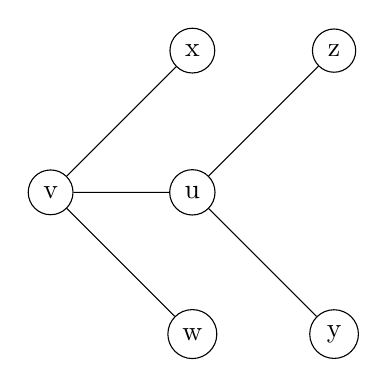
\begin{tikzpicture} 
	[main node/.style={circle, draw}, scale=1.8]
	\node[main node]  (v) at (0, 1) {v}; 
	\node[main node]  (w) at (1, 0) {w};
	\node[main node]  (u) at (1, 1) {u};
	\node[main node]  (x) at (1, 2) {x};
	\node[main node]  (y) at (2, 0) {y};
	\node[main node]  (z) at (2, 2) {z};
	\path (v) edge node {} (w);
	\path (v) edge node {} (u);
	\path (v) edge node {} (x);
	\path (u) edge node {} (y);
	\path (u) edge node {} (z);
	\end{tikzpicture}
	\label{fig:example_coverage}
	\caption{Coverage}
\end{figure}
\newline\underline{Stap \ref{itm:sort}}: Het eigenlijke sorteren van de SortedNodeArray gebeurt tijdens deze stap. De toppen worden gesorteerd in stijgende graad. Dit is een optimalisatie op het eigenlijke algoritme zodat het algoritme beter en sneller presteert. Deze SortedNodeArray heeft 3 methodes: toppen toevoegen, sorteren en de gesorteerde toppen opvragen. Dit zijn de enige vereisten. Het toevoegen van de toppen gebeurt tijdens het inlezen van de data en het sorteren van de toppen gebeurt \'{e}\'{e}nmalig bij het begin van het algoritme. Vervolgens kunnen de gesorteerde toppen altijd opgevraagd waarden verder in het algoritme, deze array verandert niet tijdens het algoritme. Enkel de coverage van de elementen is variabel. Als laatste wil ik de nadruk leggen op het feit dat deze stap een optimalisatie is. Het algoritme zou perfect werken, maar met iets slechtere prestaties zonder deze stap.
\newline\underline{Stap \ref{itm:degree1}}: Dit is ook een optimalisatie op het eigenlijke algoritme. Indien een top graad 1 heeft, weten we zeker dat de buur van deze top moet toegevoegd worden aan de dominante lijst aangezien de top enkel op deze manier bereikt kan worden. 
\newline\underline{Stap \ref{itm:actualalg}}: Deze stap voegt telkens toppen toe met een werkelijke bedekking groter dan een zeker getal. Dit getal start met 6 en decrementeert na elke iteratie van deze stap. Het algoritme zou ook werken indien er \'{e}\'{e}n iteratie is met minimum bedekking 1. Echter, het algoritme levert betere prestaties door eerst alle toppen toe te voegen die een hogere bedekking hebben, en vervolgens toppen met een kleinere bedekking.  Voor de duidelijkheid wordt het minimale algoritme, m.a.w. het algoritme die een dominante lijst produceert zonder de voorgaande optimalisaties, beschreven in algoritme \ref{alg:minimaldominantie}. Enkele belangrijke optimalisaties in het algoritme: 
\begin{itemize}
	\item Lijn \ref{step:opt1}: Als de coverage van de top gelijk is aan 0. Is het beter om bij een andere top lokaal te zoeken. 
	\item Lijn \ref{step:opt2}: Als de bedekking (bovengrens van de werkelijke bedekking) van een top 0 is, heeft het geen zin om deze top verder te bekijken. 
	\item Lijn \ref{step:opt3}: Als de werkelijke bedekking van een top gelijk is aan 0, heeft het ook geen zin om deze toe te voegen. 
\end{itemize}
Al deze optimalisaties verhinderen dat slechte toppen zouden toegevoegd worden. In het eigenlijke algoritme, wordt vergeleken in deze stappen met een minimum. Dit is echter niet nodig, maar zorgt wel voor betere prestaties. De enige vereiste van het algoritme is, dat de stap die beschreven wordt door algoritme \ref{alg:minimaldominantie} uitgevoerd wordt. In de implementatie wordt bij het bekijken van de nabuurschap van een top over de bogen ge\"{i}tereerd van de top. De top zelf bevat namelijk een List datastructuur die alle adjecente bogen bevat van de top. Ook wordt een variabele bijgehouden die het bereik van de dominante lijst bijhoudt. Zodra dit gelijk is aan $|V(G)|$ kan het algoritme eindigen. Als laatste wordt ook een boolean visited bijgehouden bij elke top. Een top wordt bezocht zodra hij of een buur wordt toegevoegd aan de dominante lijst. Eens een buur bezocht is, kan hij geen verdere bijdrage leveren tot het vergroten van het bereik van de dominante lijst. De implementatie van het bezoeken van een top verzekerd dat, indien een top nog niet bezocht werd, zijn coverage decrementeerd. 
\begin{tcolorbox}[blanker,float=btp, grow to left by=2cm,grow to right by=2cm]
	\begin{algoritme}
		\caption{Dominante verzameling van vlakke grafen}
		\begin{algorithmic}
			\Require Een planaire graaf G(V(G),E(G))
			\Ensure Een dominante verzameling D
			\State $totalCoverage \gets 0$
			\State $ i \gets 0$
			\While{$totalCoverage < |V(G)|$}
			\State $v \gets v_i \in V(G)$
			\If{$coverage(v) > 0$}\label{step:opt1}
			\State Neem $max\ |\ (\forall u \in \{v\} \cup N_G(v)) \land (max \ne u) \Rightarrow coverage(max)>coverage(u))$
			\If{$coverage(max) > 0$}\label{step:opt2}
			\State actualCoverage $\gets \{w\ |\ w  \in \{max\} \cup N_G(max) \land w\ niet \  bezocht\}$
			\If{$actualCoverage > 0$}\label{step:opt3}
			\State $totalCoverage \gets totalCoverage + actualCoverage$
			\State $coverage(max)  \gets 0$
			\State $ D \cup \{max\}$
			\State Bezoek max en zijn buren
			\EndIf 
			\EndIf
			\EndIf
			\State $i \gets i+1$
			\EndWhile		
		\end{algorithmic}
		\label{alg:minimaldominantie}
	\end{algoritme}
\end{tcolorbox}
\FloatBarrier
\subsubsection{Experimenten}
\paragraph{Optimalisaties}
Bij de experimenten omtrent optimalisaties gebruik ik steeds de gegeven testsets om het nut van een optimalisatie te testen. Er wordt (onder andere) vergeleken tussen een uitvoering zonder de optimalisatie en met de optimalisatie. De tabellen zijn telkens als volgt geformatteerd:
Bij de uitvoering van het algoritme onder de toestand beschreven in de bovenste kolommen heeft de graaf, gelezen uit graaf.sec, $x/y$\% toppen met x = $|D|$ (D = dominante lijst) en y = $|V(G)|$ Een cel is groen indien onder de huidige optie het algoritme de beste opties geeft voor graaf.sec. De exacte implementaties gebruik per algoritme kunnen gevonden worden in de Java-code.
\subparagraph{Sorteren} De variabele is hier de ordening van de toppen V(G) gebaseerd op hun graad. Er zijn 3 mogelijkheden: stijgende volgorde, dalende volgorde of willekeurige volgorde.  In tabel \ref{tabel:ordening} kan je zien dat bij elke graaf een dalende volgorde de beste resultaten teruggeeft. Een dalende volgorde betekent: indien we de toppen overloppen van index 0, worden de graad van elke top telkens kleiner. Aangezien deze optie de beste resultaten teruggeeft, wordt dit ook gebruikt. 



\subparagraph{Toppen met hoge minimumbedekking eerst}
Indien telkens opnieuw het algoritme uitgevoerd wordt, geeft dit betere resultaten als toppen met hogere minimum werkelijke bedekking eerst worden toegevoegd. Bij het eerste experimenten testen we wanneer het algoritme het beste presteert als telkens eerst toppen met een zekere werkelijke bedekking worden toegevoegd, en dit iteratief gebeurt met decrementerende minimale werkelijke bedekking. Graaf5.sec tot graaf8.sec laten we hier buiten beschouwing aangezien deze telkens even goed presteren. In tabel \ref{tabel:bedekking1} en \ref{tabel:bedekking2} zie je de resultaten van het uitvoeren van het algoritme vanaf een zekere werkelijke bedekking. De prestatie van een zekere minimale bedekking is zeer variabel van graaf tot graaf, het gemiddelde balanceert rond beginnen met een minimale bedekking van 7. Uit tabel \ref{tabel:bedekking3} kan geconcludeerd worden dat minimale bedekking 6 in het geheel de beste minimale dominante verzamelingen levert. Dit optimalisatieniveau wordt ook gebruikt in het algoritme.

\subparagraph{Toppen met graad 1}
In dit experiment wordt getest wat het effect is van het vooraf toevoegen van buren met toppen van graad 1. Hierbij worden de optimale instellingen verkregen uit vorige experimenten gebruikt. In tabel \ref{table:oneneighbour} kunnen de resultaten bekeken worden van het experiment. De optimalisatie zorgt telkens voor betere resultaten. Vooral bij graaf5.sec tot en met graaf8.sec is er een merkwaardig verschil. De grafen kunnen hier namelijk volledig opgebouwd worden door het toevoegen van de buren van toppen met graad 1. Deze optimalisatie is dus zeker helpvol en kan veel onnodig rekenwerk besparen.

\subparagraph{Niet-lineair gretig algoritme}
Als laatste bekijk ik het effect van het gebruik van een bovengrens (benadering) van de werkelijke coverage. Hiervoor heb ik het algoritme ge\"{i}mplementeerd, maar in de plaats van getCoverage() wordt nu getActualCoverage() gebruikt. Dit is de som van het aantal onbezochte buren en zichzelf indien de top nog niet bezocht werd. Op figuur \ref{tabel:nonlinear} kan je zien dat het algoritme weliswaar altijd minstens even goed presteert. Het verschil is echter merkwaardig klein. Het niet-lineaire algoritme presteert hoogstens 0.5\% beter. 

\begin{table}
	\centering
	\begin{tabular}{|l|c|c|c|}
		\hline
		& \multicolumn{3}{c|}{Ordening}		\\ \hline
		Graaf & Geen ordening  & Stijgende volgorde  & Dalende volgorde 		\\ \hline
		graaf1.sec & 20,44\% & 20,55\% &  \cellcolor{LimeGreen}19,98\%		\\ \hline
		graaf2.sec & 19,04\% & 19,02\% &  \cellcolor{LimeGreen}18,64\%		\\ \hline
		graaf3.sec & 21,10\% & 20,98\% &  \cellcolor{LimeGreen}20,87\%		\\ \hline
		graaf4.sec & 19,80\% & 19,76\% &  \cellcolor{LimeGreen}19,48\%		\\ \hline
		graaf5.sec &  \cellcolor{LimeGreen}33,33\% & 33,33\% & 33,33\%		\\ \hline
		graaf6.sec &  \cellcolor{LimeGreen}33,33\% & 33,33\% & 33,33\%		\\ \hline
		graaf7.sec &  \cellcolor{LimeGreen}33,33\% & 33,33\% & 33,33\%		\\ \hline
		graaf8.sec &  \cellcolor{LimeGreen}33,33\% & 33,33\% & 33,33\%		\\ \hline
		triang1.sec & 17,16\% & 17,09\% &  \cellcolor{LimeGreen}16,72\%		\\ \hline
		triang2.sec & 16,90\% & 16,77\% &  \cellcolor{LimeGreen}16,58\%		\\ \hline
	\end{tabular}
	\caption{Ordening van de toppen}
	\label{tabel:ordening}
\end{table}

\begin{table}
	\centering
	\begin{tabular}{|l|c|c|c|c|c|c|c|c|}
		\hline
		& \multicolumn{8}{c|}{Minimum Bedekking}		\\ \hline
		Graaf & 0  & 1  & 2  & 3  & 4  & 5  & 6  & 7 		\\ \hline
		graaf1.sec & 22,39\% & 20,98\% & 20,38\% & 20,06\% & 20,05\% &  \cellcolor{LimeGreen}19,98\% & 19,98\% & 20,00\%		\\ \hline
		graaf2.sec & 21,10\% & 19,82\% & 19,24\% & 18,92\% & 18,70\% & 18,66\% &  \cellcolor{LimeGreen}18,64\% & 18,66\%		\\ \hline
		graaf3.sec & 23,27\% & 21,81\% & 21,22\% & 20,99\% & 20,92\% & 20,89\% & 20,87\% &  \cellcolor{LimeGreen}20,84\%		\\ \hline
		graaf4.sec & 21,81\% & 20,61\% & 20,01\% & 19,70\% & 19,54\% & 19,49\% &  \cellcolor{LimeGreen}19,48\% & 19,50\%		\\ \hline
		graaf5.sec &  \cellcolor{LimeGreen}33,33\% & 33,33\% & 33,33\% & 33,33\% & 33,33\% & 33,33\% & 33,33\% & 33,33\%		\\ \hline
		graaf6.sec &  \cellcolor{LimeGreen}33,33\% & 33,33\% & 33,33\% & 33,33\% & 33,33\% & 33,33\% & 33,33\% & 33,33\%		\\ \hline
		graaf7.se c &  \cellcolor{LimeGreen}33,33\% & 33,33\% & 33,33\% & 33,33\% & 33,33\% & 33,33\% & 33,33\% & 33,33\%		\\ \hline
		graaf8.sec &  \cellcolor{LimeGreen}33,33\% & 33,33\% & 33,33\% & 33,33\% & 33,33\% & 33,33\% & 33,33\% & 33,33\%		\\ \hline
		triang1.sec & 19,03\% & 17,82\% & 17,25\% & 17,06\% & 16,86\% & 16,75\% & 16,72\% &  \cellcolor{LimeGreen}16,69\%		\\ \hline
		triang2.sec & 18,81\% & 17,67\% & 17,15\% & 16,85\% & 16,71\% & 16,61\% & 16,58\% &  \cellcolor{LimeGreen}16,57\%		\\ \hline
	\end{tabular}
	\caption{Minimale bedekking van de toppen.}
	\label{tabel:bedekking1}
\end{table}

\begin{table}[tbp]
	\centering
	\begin{tabular}{|l|c|c|c|c|c|c|c|c|}
		\hline
		& \multicolumn{8}{c|}{Minimum Bedekking}		\\ \hline
		Graaf & 8  & 9  & 10  & 11  & 12  & 13  & 14  & 15 		\\ \hline
		graaf1.sec &  \cellcolor{LimeGreen}20,13\% & 20,18\% & 20,22\% & 20,24\% & 20,22\% & 20,19\% & 20,19\% & 20,19\%		\\ \hline
		graaf2.sec & 18,70\% &  \cellcolor{LimeGreen}18,69\% & 18,70\% & 18,71\% & 18,71\% & 18,70\% & 18,69\% & 18,70\%		\\ \hline
		graaf3.sec &  \cellcolor{LimeGreen}20,78\% & 20,80\% & 20,82\% & 20,82\% & 20,81\% & 20,78\% & 20,78\% & 20,78\%		\\ \hline
		graaf4.sec & 19,51\% & 19,50\% &  \cellcolor{LimeGreen}19,49\% & 19,51\% & 19,51\% & 19,50\% & 19,49\% & 19,50\%		\\ \hline
		graaf5.sec &  \cellcolor{LimeGreen}33,33\% & 33,33\% & 33,33\% & 33,33\% & 33,33\% & 33,33\% & 33,33\% & 33,33\%		\\ \hline
		graaf6.sec &  \cellcolor{LimeGreen}33,33\% & 33,33\% & 33,33\% & 33,33\% & 33,33\% & 33,33\% & 33,33\% & 33,33\%		\\ \hline
		graaf7.sec &  \cellcolor{LimeGreen}33,33\% & 33,33\% & 33,33\% & 33,33\% & 33,33\% & 33,33\% & 33,33\% & 33,33\%		\\ \hline
		graaf8.sec &  \cellcolor{LimeGreen}33,33\% & 33,33\% & 33,33\% & 33,33\% & 33,33\% & 33,33\% & 33,33\% & 33,33\%		\\ \hline
		triang1.sec &  \cellcolor{LimeGreen}16,73\% & 16,76\% & 16,77\% & 16,76\% & 16,75\% & 16,74\% & 16,75\% & 16,76\%		\\ \hline
		triang2.sec & 16,57\% & 16,56\% & 16,56\% & 16,55\% & 16,54\% & 16,52\% & 16,53\% &  \cellcolor{LimeGreen}16,52\%		\\ \hline
	\end{tabular}
	\caption{Minimale bedekking van de toppen.}
	\label{tabel:bedekking2}
\end{table}

\begin{table}
	\centering
	\begin{tabular}{|c|c|}
		\hline
		Minimum bedekking & $|D|\ /\ |V(G)|$		\\ \hline
		0 & 25,0729\% \\ \hline
		1 & 24,2659\% \\ \hline
		2 & 23,8922\% \\ \hline
		3 & 23,6965\% \\ \hline
		4 & 23,5913\% \\ \hline
		5 & 23,5475\% \\ \hline
		6 &\cellcolor{LimeGreen} 23,5370\% \\ \hline
		7 & 23,5413\% \\ \hline
		8 & 23,5541\% \\ \hline
		9 & 23,5519\% \\ \hline
	\end{tabular}
	\caption{Aantal toppen in alle dominante verzamelingen t.o.v. aantal toppen in alle grafen.}
	\label{tabel:bedekking3}
\end{table}

\begin{table}
	\centering
	\begin{tabular}{|l|c|c|}
		\hline
		& \multicolumn{2}{c|}{Toppen van graad 1}		\\ \hline
		Graaf & Zonder optimalisatie  & Met optimalisatie 		\\ \hline
		graaf1.sec & 20,03\% &  \cellcolor{LimeGreen}19,98\%		\\ \hline
		graaf2.sec & 18,66\% &  \cellcolor{LimeGreen}18,64\%		\\ \hline
		graaf3.sec & 21,01\% &  \cellcolor{LimeGreen}20,87\%		\\ \hline
		graaf4.sec & 19,60\% &  \cellcolor{LimeGreen}19,48\%		\\ \hline
		graaf5.sec & 38,72\% &  \cellcolor{LimeGreen}33,33\%		\\ \hline
		graaf6.sec & 38,65\% &  \cellcolor{LimeGreen}33,33\%		\\ \hline
		graaf7.sec & 38,67\% &  \cellcolor{LimeGreen}33,33\%		\\ \hline
		graaf8.sec & 38,60\% &  \cellcolor{LimeGreen}33,33\%		\\ \hline
		triang1.sec &  \cellcolor{LimeGreen}16,72\% & 16,72\%		\\ \hline
		triang2.sec &  \cellcolor{LimeGreen}16,58\% & 16,58\%		\\ \hline
	\end{tabular}
	\caption{Experiment met betrekking tot het al dan niet toevoegen van buren van toppen met graad 1.}
	\label{table:oneneighbour}
\end{table}

\begin{table}
	\centering
	\begin{tabular}{|l|c|c|}
		\hline
		& \multicolumn{2}{c|}{Vergelijking lineair - niet lineair gretig algoritme}		\\ \hline
		Graaf & Niet-lineair  & Lineair 		\\ \hline
		graaf1.sec &  \cellcolor{LimeGreen}19,57\% & 19,98\%		\\ \hline
		graaf2.sec &  \cellcolor{LimeGreen}18,16\% & 18,64\%		\\ \hline
		graaf3.sec &  \cellcolor{LimeGreen}20,50\% & 20,87\%		\\ \hline
		graaf4.sec &  \cellcolor{LimeGreen}19,05\% & 19,48\%		\\ \hline
		graaf5.sec &  \cellcolor{LimeGreen}33,33\% & 33,33\%		\\ \hline
		graaf6.sec &  \cellcolor{LimeGreen}33,33\% & 33,33\%		\\ \hline
		graaf7.sec &  \cellcolor{LimeGreen}33,33\% & 33,33\%		\\ \hline
		graaf8.sec &  \cellcolor{LimeGreen}33,33\% & 33,33\%		\\ \hline
		triang1.sec &  \cellcolor{LimeGreen}16,47\% & 16,72\%		\\ \hline
		triang2.sec &  \cellcolor{LimeGreen}16,17\% & 16,58\%		\\ \hline
	\end{tabular}
	\caption{Vergelijking implementaties}
	\label{tabel:nonlinear}
\end{table}

\paragraph{Verschillende grafen}
In dit onderdeel ga ik in op enkele voorbeeldgrafen en bespreek ik hoe het algoritme presteert bij de gegeven grafen. 

De worst case graaf voor dominante verzamelingen is een \underline{cyclische graaf}, zodat elke top juist 2 bogen heeft en de graaf juist 1 cykel bevat. 
Elke top heeft dus graad 2. Een minimale dominante verzameling bevat dan 1/3 van de toppen van de graaf. Bij het uitvoeren van mijn algoritme op dergelijke graaf, geeft het altijd de optimale dominante verzameling terug met grootte 1/3, hier werkt het algoritme dus perfect. 
Als volgt kijken we naar grafen waarvan de buren op afstand 2 van een ideale top een groot aantal toppen heeft. Aangezien de bedekking van deze toppen niet aangepast worden door het toevoegen van een top op afstand 2, zou dit een slechtere benadering moeten geven. Een goed voorbeeld hiervan is een \underline{Petersen-graaf}. Dit is een graaf met 10 toppen en 15 bogen en wordt vaak gebruikt als tegenvoorbeeld voor vele optimistische problemen. Bij het uitvoeren van het algoritme op deze graaf, bekom ik een dominante verzameling met 3 toppen, opnieuw presteert het ideaal. 
Als laatste ik de graaf die je kan zien op figuur \ref{fig:schaakmat}
, ik benoem de graaf als de \underline{schaakmat graaf}. Het is een graaf met 8x8 toppen zodat elke top een vak uit het speelveld van een schaakmat voorstelt, en de toppen van 2 naburige vakjes verbonden zijn door een boog. Het is goed mogelijk dat mijn algoritme voor deze graaf slecht presteert, aangezien alle toppen zeer verbonden zijn, zodat de coverage een slechte benadering zal geven. De coverage van de buren op afstand 2 van een top zullen immers niet aangeraakt worden. Dit zorgt ervoor dat de dominante lijst slechtere resultaten zal bekomen. Het resultaat van mijn algoritme op de gegeven graaf kan je ook zien op figuur \ref{fig:schaakmat}. De toppen uit de dominante lijst werden in het groen gekleurd. De dominante lijst bevat $22/64$ (34\%) van de toppen. Het is moeilijk om voor een graaf van deze omvang te weten of de oplossing een goede benadering heeft. Het is makkelijker om de graaf op te delen in 4x4 vlakken. Beschouw figuur \ref{fig:schaakmat2}, een minimale dominante verzaleming wordt verkregen door de groene toppen. Dit zijn er precies 6. 
Een dominante verzameling voor een schaakmatgraaf, zou dan kunnen verkregen worden door in elke vlak juist die 4 toppen te kiezen. Dan is er een dominante verzameling van 24 toppen. Dit is een slechtere benadering dan dan de benadering van het algoritme. Een echte optimale verzameling zoeken van een graaf van dergelijke omvang is moeilijk, daarom implementeerde ik een variatie op mijn algoritme, die niet lineair werkt, maar betere benaderingen moet geven. De wijziging op het algoritme is als volgt: in de plaats van een bovengrens van de werkelijke coverage te gebruiken, wordt nu de echte coverage gebruikt zodat we in elke stap verzekeren dat de beste lokale top toegevoegd wordt. Bij het uitvoeren van het algoritme op de schaakmat graaf krijg ik een verzameling van 21 toppen. Dit is slechts 1 top minder dan het lineaire algoritme. We kunnen dus stellen dat het algoritme goede benaderingen geeft. 

\begin{figure}[tbp]
	\centering
	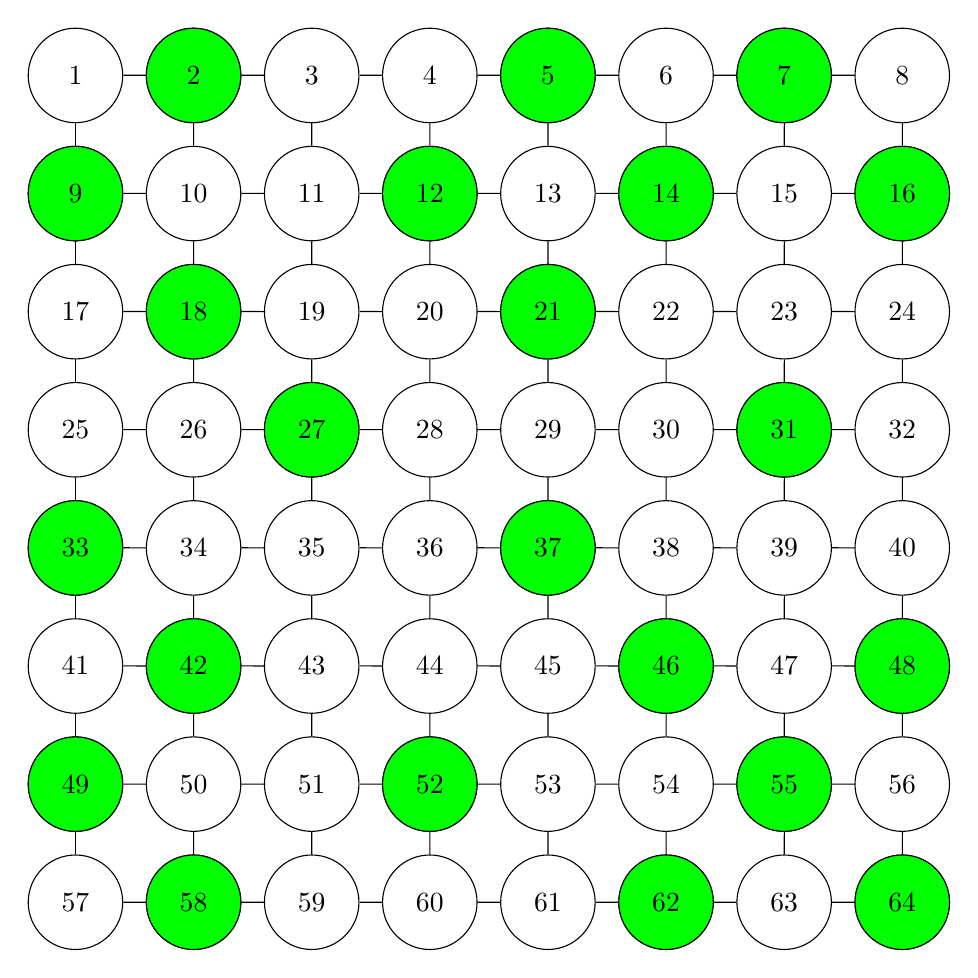
\begin{tikzpicture} 
	[main node/.style={circle, draw}, minimum width=1.2cm, minimum height=1.2cm, scale=1.5]
	\newcounter{x}
	\foreach \i in {0,1,...,7}{
		\foreach \j in {0,1,...,7}{
			\stepcounter{x};
			\node[main node]  (\arabic{x}) at (\j, 8-\i) {\arabic{x}};
		}
	}

	\setcounter{x}{8}
	\newcounter{y}
	\newcounter{z}
	\stepcounter{z}
	\foreach \i in {1,2,...,7}{
		\foreach \j in {1,2,...,7}{
			\stepcounter{y};
			\stepcounter{z};
			\stepcounter{x};
			\path (\arabic{y}) edge node {} (\arabic{z}); %right
			\path (\arabic{y}) edge node {} (\arabic{x}); %down
		}
		\stepcounter{y};
		\stepcounter{z};
		\stepcounter{x};
	}

	\setcounter{x}{57}
	\setcounter{y}{58}
	\newcounter{a}
	\newcounter{b}
	\setcounter{a}{8}
	\setcounter{b}{16}
	\foreach \i in {1,2,...,7}{
		\path (\arabic{x}) edge node {} (\arabic{y}); %right
		\path (\arabic{a}) edge node {} (\arabic{b}); %down
		\stepcounter{y};
		\stepcounter{x};
		\addtocounter{a}{8};
		\addtocounter{b}{8};
	}	
	
	%color dominant list nodes.
	\node[main node, fill=green] (55) at (6,2) {55};
	\node[main node, fill=green] (52) at (3,2) {52};
	\node[main node, fill=green] (42) at (1,3) {42};
	\node[main node, fill=green] (31) at (6,5) {31};
	\node[main node, fill=green] (18) at (1,6) {18};
	\node[main node, fill=green] (14) at (5,7) {14};
	\node[main node, fill=green] (37) at (4,4) {37};
	\node[main node, fill=green] (12) at (3,7) {12};
	\node[main node, fill=green] (58) at (1,1) {58};
	\node[main node, fill=green] (2) at (1,8) {2};
	\node[main node, fill=green] (16) at (7,7) {16};
	\node[main node, fill=green] (27) at (2,5) {27};
	\node[main node, fill=green] (62) at (5,1) {62};
	\node[main node, fill=green] (48) at (7,3) {48};
	\node[main node, fill=green] (33) at (0,4) {33};
	\node[main node, fill=green] (64) at (7,1) {64};
	\node[main node, fill=green] (49) at (0,2) {49};
	\node[main node, fill=green] (7) at (6,8) {7};
	\node[main node, fill=green] (9) at (0,7) {9};
	\node[main node, fill=green] (5) at (4,8) {5};
	\node[main node, fill=green] (46) at (5,3) {46};
	\node[main node, fill=green] (21) at (4,6) {21};
	\end{tikzpicture}
	\caption{Een schaakmatgraaf}
	\label{fig:schaakmat}
\end{figure}

\begin{figure}[tbp]
	\centering
	\begin{tikzpicture} 
	[main node/.style={circle, draw}, minimum width=1.2cm, minimum height=1.2cm, scale=1.5]
	\setcounter{x}{0}
	\foreach \i in {0,1,...,3}{
		\foreach \j in {0,1,...,3}{
			\stepcounter{x};
			\node[main node]  (\arabic{x}) at (\j, 4-\i) {\arabic{x}};
		}
	}
	
	\setcounter{x}{4}
	\setcounter{y}{0}
	\setcounter{z}{1}
	\foreach \i in {1,2,3}{
		\foreach \j in {1,2,3}{
			\stepcounter{y};
			\stepcounter{z};
			\stepcounter{x};
			\path (\arabic{y}) edge node {} (\arabic{z}); %right
			\path (\arabic{y}) edge node {} (\arabic{x}); %down
		}
		\stepcounter{y};
		\stepcounter{z};
		\stepcounter{x};
	}
	
	\setcounter{x}{13}
	\setcounter{y}{14}
	\setcounter{a}{4}
	\setcounter{b}{8}
	\foreach \i in {1,2,3}{
		\path (\arabic{x}) edge node {} (\arabic{y}); %right
		\path (\arabic{a}) edge node {} (\arabic{b}); %down
		\stepcounter{y};
		\stepcounter{x};
		\addtocounter{a}{4};
		\addtocounter{b}{4};
	}	
	\node[main node, fill=green] (1) at (0,4) {1};
	\node[main node, fill=green] (6) at (1,3) {6};
	\node[main node, fill=green] (11) at (2,2) {11};
	\node[main node, fill=green] (16) at (3,1) {16};
	\node[main node, fill=green] (4) at (3,4) {4};
	\node[main node, fill=green] (13) at (0,1) {13};
	
	\end{tikzpicture}
	\caption{Een 4x4 schaakmatgraaf}
	\label{fig:schaakmat2}
\end{figure}

\paragraph{Conlusie}
Desondanks het feit dat dit algoritme werkt met benaderingen voor de werkelijke bedekking, presteert het bijna even goed als een algoritme waarbij gewerkt wordt met werkelijke bedekkingen. Ook is het zeer moeilijk om een graaf te vinden waarbij het algoritme faalt. Ik denk dus dat het moeilijk is om een gretig lineair algoritme te vinden die veel beter presteert dan het huidige algoritme. 

\subsection{Hamiltoniaanse cykels in vlakke triangulaties}
\paragraph{Algemeen}
Het algoritme dat ik gebruik om hamiltoniaanse cykels te bepalen wordt beschreven in algoritme \ref{alg:hamilton}. Eerst en vooral wil ik vermelden dat de berekening van de Yutsis-decompositie in dit algoritme gebaseerd werd op het onderdeel "Een voorbeeld: het Yutsis probleem"\ uit de cursus, en verder werd aangevuld met eigen inbreng en ook een aantal idee\"{e}n uit de paper "To be or not to be Yutsis". Mijn algoritme gaat uit van de eigenschap bewezen in theoretische vraag 2.  De eigenschap gaat als volgt: In de hamiltoniaanse cykel van een vlakke triangulatie zijn er evenveel vlakken binnen en buiten de cykel. Volgens deze eigenschap volstaat het om 2 verzamelingen met vlakken te zoeken zodat de ene verzameling alle vlakken bevat buiten de cykel en de overige verzameling alle vlakken bevat binnen de cykel. Om dergelijke verzameling te zoeken, maak ik een duale graaf van de vlakke triangulatie. In deze duale graaf zijn alle vlakken uit de triangulatie toppen. Twee toppen zijn verbonden met een boog als de vlakken voorgesteld door de toppen een gemeenschappelijke boog hebben en dus aanliggend zijn. Deze duale-graaf is een 3-reguliere graaf aangezien elk vlak in een vlakke triangulatie juist 3 aanliggende vlakken heeft aan zijn 3 bogen. Een belangrijke eigenschap van dergelijke verzameling van vlakken is dat deze vlakken een boom moeten vormen in de duale graaf zoals besproken in lemma \ref{lemma1}. Een dergelijke decompositie van een graaf in twee onafhankelijke bomen van gelijke grootte heet een Yutsis-decompositie. Eens de 2 onafhankelijke verzamelingen van vlakken gevonden werd is het eenvoudig om een cykel te vinden. Het volstaat om elke gemeenschappelijke boog van twee vlakken uit een verschillende verzameling toe te voegen aan de cykel. 
Het algoritme bestaat dus uit 3 belangrijke delen:
\begin{itemize}
	\item Het maken van de duale graaf van de vlakke triangulatie. 
	\item Het berekenen van een Yutsis-decompositie van deze duale graaf. 
	\item Het berekenen van cykels m.b.v. de Yutsis-decompositie indien \'{e}\'{e}n gevonden werd. 
\end{itemize}
Nu zal ik op de implementatie van elk onderdeel dieper ingaan. 
\paragraph{De duale graaf}
De grootste moeilijkheid bij de duale graaf is om de vlakken van de vlakke triangulatie correct te bepalen en voor elk vlak zijn buren toe te voegen. 
Initieel zou ik dit op een recursieve manier implementeren, maar al snel bleek dit niet te werken voor grote grafen omdat de recursie te ver ging. 
\\\\Het opbouwen van de duale graaf begint door het nemen van een boog en zijn aanliggende vlakken van een boog toe te voegen aan een array. Vervolgens worden de vlakken van de array overlopen. Van elk vlak worden zijn aanliggende toppen toegevoegd. (De array wordt dus groter tijdens het itereren.) Eens elke vlak bekeken werd uit de array, inclusief de nieuwe vlakken, is de duale graaf compleet. Het toevoegen van de aanliggende vlakken van een vlak gaat als volgt. Itereer over de bogen van het huidige vlakken en bepaal het andere aanliggende vlak. Dit vlak voeg je toe in de lijst met alle vlakken en in de lijst van aanliggende vlakken van het huidige vlak. Hiernaast wordt ook het huidige vlak toegevoegd aan de lijst van aanliggende vlakken van het nieuwe vlak. Indien het vlak al bestond update je enkel de aanliggende buurlijsten van de beide vlakken (dit kan snel gecontroleerd worden door de aanliggende vlakken van een boog ook bij te houden). 
\\\\Een aanliggend vlak aan een boog kan gevonden worden door het bekijken van zijn vorige en volgende boog ten opzichte van zijn eindpunten. De volgende en vorige boog van een boog t.o.v. van \'{e}\'{e}n van zijn toppen wordt op zijn beurt bepaald als volgt: voor het eindpunt van de boog wordt de index van deze boog in de lijst van bogen van het eindpunt opgeslagen. De volgende of vorige boog wordt dan gevonden op de index van die boog in het eindpunt resp. plus of min \'{e}\'{e}n. De reden hiervoor is dat de bogen op een circulaire manier worden opgeslagen in de toppen, dus de vorige en volgende boog in de lijst van adjecente bogen van de top wordt simpelweg bepaald door de boog op de volgende of vorige index te nemen t.o.v. de index van de gegeven boog.
\\\\Eens alle toppen en de buren van elke top in de vlakke graaf bepaald werden (de vlakken in de vlakke triangulatie), worden de paren van bogen gemaakt in de duale graaf, omdat dit verder in het algoritme snel moet kunnen opgevraagd worden. Dit wordt gedaan door een 3-dubbele for-lus. In de buitenste lus wordt ge\"{i}tereerd over elke top v van de duale graaf. In de lus hierbinnen wordt ge\"{i}tereerd over elke buur w van v. In de lus hier nog eens binnen wordt ge\"{i}tereerd over elke buur u van w. Alle toppen zodat v $\neq$ u impliceren dan een paar van bogen waarbij v en w de eindpunten zijn en w het centrum. Merk op dat deze 3-dubbele for-lus lineair werkt. De buitenste for-lus itereert juist n keer, met n het aantal vlakken. De binnenste for-lussen itereren elk 3 keer omdat elke top in de 3-reguliere graaf juist 3 buren heeft. Dit zorgt dus voor een totaal van $3*3*n = 9*n$ iteraties. In elke top worden juist 3 paren opgeslagen, de paren waarvan de top het centrum is. 
\\\\Als laatst worden alle vlakken van de duale graaf gemaakt. Deze vlakken zijn namelijk ook noodzakelijk om het eigenlijke algoritme goed te laten presteren. Opnieuw, net als bij het bepalen van vlakken in vlakke triangulaties, is er nood aan een circulaire volgorde van de buren van toppen in de duale graaf. De bogen van een vlak worden in circulaire opgeslagen in het vlak. Nu is het eenvoudig om ook deze volgorde aan te nemen voor de buren van een vlak (aangezien elke boog een naburig vlak impliceert). Hiernaast wordt in elk paar van de boog een richting opgeslagen. Dit vertelt of de index van het centrum met \'{e}\'{e}n verhoogd of verlaagd moet worden van de index van een eindpunt om het andere eindpunt te verkrijgen. Nemen we de twee vorige ide\"{e}en, is het mogelijk om te starten in een paar en alle toppen in een vlak te overlopen door steeds eenzelfde richting, namelijk de richting bepaald door het paar, te nemen.  We kiezen telkens de index van de vorige top plus of min \'{e}\'{e}n afhankelijk van de richting van het paar. Bij het bepalen van alle vlakken aan elk paar ook het juiste vlak toegekend, zodat een vlak snel vanuit een paar kan gevonden worden. 
\paragraph{De Yutsis-decompositie}
\label{sec:yutsus}
Nu de duale graaf berekend is, kan het effectieve algoritme beginnen. Er moeten 2 onafhankelijke toppenverzamelingen gemaakt worden met gelijke lengte en waarvan de deelgrafen ge\"{i}mpliceerd door deze verzameling toppen zijn. 
\\\\Voor dit algoritme heb ik mijn eigen datastructuur ge\"{i}mplenteerd die een toppenverzameling voorstelt. Deze datastructuur kan toevoegen, verwijderen, opzoeken en controleren van de aanwezigheid van een top in constante tijd. Het algoritme is mogelijk zonder dergelijke array, maar er zouden bepaalde optimalisaties niet mogelijk zijn. (Bijvoorbeeld het verwijderen van toppen uit V). Deze constante tijden worden mogelijk gemaakt door het bijhouden van de huidige array van een top (aangezien elke top zich maar in \'{e}\'{e}n verzameling kan bevinden op een moment in het algoritme). Hiernaast wordt ook de index bijgehouden voor constant verwijderen en opzoeken.
Intern bevat de PlaneNodeArray een array van PlaneNodes, deze stellen op zich toppen voor in de duale graaf. Het algoritme simuleert een stack en probeert het laatst toegevoegde element terug te geven bij een pull operatie. Dit is echter niet altijd mogelijk aangezien de elementen veel van plaats verschuiven. Na het toevoegen van 1 element en het verwijderen van 2 elementen van deze lijst wordt slechts een benadering gegeven van het laatst toegevoegde element. Dit zou dan \'{e}\'{e}n van de laatst toegevoegde elementen zijn. Het algoritme presteert beter met de PlaneNodeArray dan bij het gebruik van een echte stack en/of arraylist omdat ook aanwezigheid controleren, opzoeking en verwijderen allemaal in constante tijd kan gebruiken, waardoor meer operaties mogelijk gemaakt worden die gebruikt kunnen worden in het algoritme.
\\\\Het algoritme werkt nu als volgt. Er worden 6 verzamelingen gemaakt, L[0],L[1],L[2], V, M en nonVisitable. Elke verzameling heeft zijn eigen betekenis: 
\begin{itemize}
	\item V bevat initieel alle toppen. Tijdens het algoritme worden hieruit enkel toppen verwijderd. Deze verzameling bevat altijd het complement van alle toppen die niet tot V behoren. 
	\item L[x] bevat alle toppen met x buren in V. Een top wordt toegevoegd tot een zekere L verzameling zodra een buur wordt toegevoegd aan M en deze top zich in de verzameling V bevindt. Het is mogelijk dat een top niet behoort tot de correcte verzameling als $x>0$ als zijn buren in V ge\"{u}pdatet worden waardoor ze niet meer tot V behoren. ($x \in [0,2]$)
	\item M: deze verzameling van toppen induceert op elk moment een deelgraaf die een boom is. Dit is \'{e}\'{e}n van de twee verzamelingen van de Yutsis-decompositie zodra $|M|=n/2$ met n de grootte van de duale graaf. 
	\item nonVisitable bevat alle toppen waarvan ondervonden is dat het nooit mogelijk is om deze top aan M toe te voegen. 
\end{itemize} 
	Het algoritme begint met het kiezen van een willekeurige top uit V en deze te wisselen (wisselen = verwijderen uit huidige en toevoegen aan nieuwe verzameling) naar de nieuwe verzameling. Zijn buren worden toegevoegd aan L[2] en alle paren uit de vlakken van de paren waarvan de toegevoegde top het centrum is, worden gemarkeerd. Nu wordt er ge\"{i}tereerd tot M volledig is ($|M| = n$) of L leeg is. 
	\\\\Binnenin deze while-lus wordt eerst een goeie kandidaat bepaald om toe te voegen aan M met juist 1 buur in M die het laatst werd toegevoegd en een maximaal aantal buren in V heeft. Deze wordt bepaald door het itereren over de toppen in L[x] startend met $x=2$,  en x te verlagen indien een zekere L[x] leeg is. Dit doe je tot je een goeie top gevonden hebt of tot alle arrays leeg zijn. In het tweede geval eindigt het algoritme. Bij het itereren over de arrays zoekend naar een goeie top kijken we telkens als $x > 0$ of het aantal buren in V correct ingesteld is, indien dit niet het geval is wordt de top in de correcte L[x] geplaatst. De nieuwe index zal altijd lager zijn dan de huidige x aangezien er nooit toppen worden toegevoegd aan V. Zodra een top gevonden wordt, wordt zijn aantal buren in M gecontroleerd, indien dit groter dan 1 is, zorgt het toevoegen van deze top aan M voor een cykel. Als dit het geval is, wordt deze top gewisseld naar nonVisitable omdat het aantal M buren nooit zal verlagen (M groeit alleen maar). Vervolgens wordt verder ge\"{i}tereerd indien geen goeie kandidaat werd gevonden, echter als een goeie kandidaat werd gevonden, wordt gecontroleerd of het toevoegen van deze top aan M ervoor zou zorgen dat de deelgraaf ge\"{i}nduceerd door de toppen die niet behoren tot M nog samenhangend zou zijn. Als dit niet het geval is, zouden de deelgrafen ge\"{i}nduceerd door de verzamelingen van de verkregen Yutsis-decompositie geen bomen induceren wat er op zijn beurt voor zorgt dat geen cykel zou gevonden worden. 
	\\\\Het controleren of een top de samenhangendheid verstoort gebeurt door het nemen van het paar (e,e') waarvan deze top het centrum is en zijn eindpunten niet tot M behoren. Juist 1 van de 3 paren waarvan de top het centrum is voldoet hieraan omdat deze top 1 naburige top in M heeft (zoals hiervoor bepaald) en 2 buren die niet tot M behoren. 
	Indien (e,e') gemarkeerd is, zou deze top de samenhangendheid verstoren, en wordt toegevoegd aan nonVisitable. Indien (e,e') niet gemarkeerd is, kan de top toegevoegd worden aan de verzameling M. Nu worden ook de paren van het vlak $f_G(e,e')$ gemarkeerd en de verzameling van de buren die tot L[x] of V behoren worden toegevoegd aan de correct L[x] verzameling. Merk dus op dat de buren uit L[x] hier in de correct L[x] array geplaatst worden.
	\\\\Zodra de while-lus voorbij is, wordt M teruggeven als het aantal toppen in M gelijk is aan de helft van de grootte van de graaf. De overige verzameling van de Yutsis-decompositie wordt ge\"{i}nduceerd door alle toppen die niet tot M behoren. 
\paragraph{De hamiltoniaanse cykel}
	Als laatste kan eenvoudigweg een cykel bepaald worden in de vlakke triangulatie door het itereren over de verkregen verzameling M met vlakken (de toppen in de duale graaf stelden vlakken voor in de vlakke triangulatie). Bij elk vlak wordt ge\"{i}tereerd over zijn 3 aanliggende vlakken. Indien een aanliggend vlak niet tot M behoort, moet de aanliggende boog toegevoegd worden aan de cykel. Ik werk echter niet met bogen maar met een array van CycleNodes waarbij elke CycleNode een referentie bijhoudt naar de top die hij voorstelt, en de vorige en volgende CycleNode. Bij het toevoegen van een boog aan een cykel wordt een nieuwe CycleNode aangemaakt voor elke top waarvan nog geen CycleNode bestaat. Vervolgens voegen de CycleNodes elkaar toe bij de array van lengte 2 met buren. Uiteindelijk zal een lijst met CycleNodes verkregen worden waarin elke CycleNode een correcte verwijzing heeft naar zijn volgende en vorige buur. De cykel kan dan geprint worden door het beginnen met een willekeurige top in de array en telkens de buur te kiezen die niet gelijk is aan de vorige. 
	 
\subsubsection{Optimalisaties en experimenten voor de Yutsis-decompositie}

\paragraph{3 verzamelingen voor de toppen uit L}
Hier zal ik de invloed nagaan van het gebruik van de 3 verzamelingen voor L om telkens de beste top te kiezen t.o.v. het kiezen van een willekeurige top in L. Bij het laatstgenoemde bestaat L weliswaar maar 1 uit array. De resultaten van dit experiment ziet u in tabel \ref{table:Lset}. Hier is een duidelijk verschil zichtbaar in het aantal cykels dat het gretige algoritme vindt t.o.v. het aantal cykels dat het willekeurige algoritme vindt. Dit algoritme werkt zoveel beter aangezien het kiezen van de top met het hoogst aantal buren in V ervoor zorgt dat het aantal kandidaten (de L verzameling) groter wordt, en dus M ook zal groter worden. De kans dat de Yutsis-decompositie gevonden wordt, stijgt dus enorm. Een uitgebreidere verklaring over het beter werken van een gretig algoritme t.o.v. het willekeurig algoritme vindt u onder de verklaring van het gretig van mijn algoritme onder theoretische opgave 3. 
\begin{table}[bh]
	\center
	\csvautotabular[separator=semicolon]{experiments/LSetExperiment.csv}
	\caption{Vergelijking van het algoritme waarbij de beste top telkens uit L wordt gekozen, of een willekeurige top. De getallen stellen het procent cykels gevonden ten opzichte van het aantal grafen in het gegeven bestand.
		\label{table:Lset}
	} 
\end{table}

\paragraph{Meerdere pogingen}
Indien het algoritme meerdere keren uitgevoerd wordt, telkens beginnend bij een andere vlak om de Yutsis-decompositie te berekenen, zou het logisch zijn moest het algoritme beter presteren. Hier zullen namelijk andere gretige beslissingen gemaakt worden zodat de kans groter wordt dat de juiste beslissingen genomen worden, en hierdoor een Yutsis-decompositie wordt gevonden.  Dit experiment wordt weergegeven in \ref{table:multipletrials}. 
De kolomnaam is hier het maximale aantal pogingen gebruikt door het algoritme om een cykel te vinden. Vanaf \'{e}\'{e}n extra poging merk je al een zeer groot verschil bij de hoeveelheid gevonden cykels. Het aantal gevonden cykels stijgt bijvoorbeeld bij een graaf met 12 toppen met 5,2\%. Bij een nieuwe poging worden echter alle stappen van het algoritme tenietgedaan, waardoor het volledige algoritme niet meer gretig is. Aangezien ik echter een algoritme moest maken die wel gretig is, laat ik deze optimalisatie terzijde in mijn finale implementatie. 
\begin{tcolorbox}[blanker,float=b, grow to left by=2cm,grow to right by=2cm]
	\begin{algoritme}
		\caption{Hamiltoniaanse cykels in vlakke  triangulaties (oud)}
		\label{alg:hamilton2}
		\begin{algorithmic}[1]
			\Require Een vlakke triangulatie G(V(G),E(G))
			\Require Een initieel lege cykel C
			\Ensure Een hamiltoniaanse cykel C in de vorm van een sequentie van bogen of $\emptyset$ als geen hamiltoniaanse cykel gevonden werd.
			\State V $\gets$ een willekeurig vlak in G
			\State Voeg de bogen van V toe aan de cykel
			\State Bezoek de bogen in de cykel
			\While{cykel is niet hamiltoniaans \& er zijn zichtbare bogen}
			\ForAll{zichtbaar boog e}
			\State V $\gets$ het aanliggende vlak van e die nog niet binnen de cykel is. 
			\State e',e'' $\gets$ de overige 2 bogen van V
			\State t $\gets$ het gemeenschappelijke eindpunt van e' en e''
			\If{e' en e'' niet bezocht \& t niet in de cykel}
			\State Voeg de e' en e'' toe aan de cykel
			\Comment Nu is V binnenin de cykel. 
			\State Bezoek e' en e''
			\Else 
			\State e is geen zichtbare boog meer
			\EndIf 
			\EndFor
			\EndWhile
		\end{algorithmic}
	\end{algoritme}
\end{tcolorbox}

\begin{table}[bh]
	\center
	\csvautotabular[separator=semicolon]{experiments/MultipleTrialsExperiment.csv}
	\caption{De variabele hier (kolomnaam) is het maximale aantal pogingen om een Yutsis-decompositie te vinden. De prestatie bij elk aantal wordt vergeleken. De getallen stellen het procent cykels gevonden ten opzichte van het aantal grafen in het gegeven bestand.
		\label{table:multipletrials}
	} 
\end{table}

\subsubsection{Een tweede gretig lineair algoritme}
Initieel had ik een ander algoritme om hamiltoniaanse cykels te berekenen. Dit presteerde echter niet goed genoeg waardoor ik het nieuwe en uiteindelijke algoritme heb gemaakt. Deze werd volledig ge\"{i}plementeerd, en zal ik hier kort bespreken en de prestatie vergelijken. 
\\\\Het oude algoritme wordt weergegeven in algoritme \ref{alg:hamilton2}.
Het algemene idee hier is: begin met cykel die 1 vlak insluit en probeer hier zoveel mogelijk vlakken aan toe te voegen door telkens over de bogen van de cykel te itereren en indien mogelijk aanliggende vlakken die niet in de cykel zijn in te voegen in de cykel terwijl de cykel blijft voldoen aan de eigenschappen van een cykel. Er zijn in het effectieve algoritme enkele toevoegen om het algoritme lineair te houden. Er wordt gewerkt met zichtbare bogen zodat elke boog juist een keer wordt bekeken om een aanliggend vlak toe te voegen. Het nut van het bezoeken van bogen is om snel te kunnen bekijken of een boog kan toegevoegd worden aan de cykel aangezien een top uit de cykel maar het eindpunt mag zijn van 2 bogen in de cykel. 
\\\\Dit algoritme presteert slechter dan het nieuwe algoritme. De resultaten van de kleine testgrafen kunnen bekeken worden in tabel \ref{table:oldhamilton}. Tot en met grafen met 8 toppen vinden beide algoritmes altijd een cykel. Echter het aantal cykels die niet gevonden worden vanaf grootte 8 stijgt veel sneller bij het oude algoritme in vergelijking met het nieuwe algoritme. Dit valt te verklaren door het feit dat het oude algoritme veel sneller kan vastlopen dan het nieuwe algoritme. Eens slechte bogen toegevoegd worden, is het zeer onwaarschijnlijk (behalve bij zeer kleine grafen), dat het algoritme nog een cykel vindt. Het nieuwe algoritme daarentegen heeft veel betere voorwaarden voor het toevoegen van vlakken, waardoor de kans op het vinden van een cykel veel groter is dan het oude algoritme. 
\newline
\begin{table}
	\center
	\csvautotabular[separator=semicolon]{experiments/oldHamiltonExperiment.csv}
	\caption{Vergelijking van algoritme \ref{alg:hamilton} (nieuw algoritme) en algoritme \ref{alg:hamilton2}  (oud algoritme). De getallen stellen het procent cykels gevonden ten opzichte van het aantal grafen in het gegeven bestand.
	\label{table:oldhamilton}
	} 
\end{table}
\subsubsection{Testgrafen}
Als laatste zal ik de prestatie bespreken van algoritme \ref{alg:hamilton} bij grote grafen. Aangezien een hamiltoniaanse cykel altijd gevonden kan worden eens de Yutsis-decompositie gevonden wordt, bespreek ik enkel de prestatie van de Yutsis-decompositie. De Yutsis-decompositie eindigt als $|M| = |V(DG)|/2$ met M de toppenverzameling uit het algoritme en DG de duale graaf uit dit algoritme. Een goeie maatstaf voor de prestatie van het algoritme is dus hoe groot M wordt voor het algoritme eindigt. De resultaten kan je vinden in tabel \ref{table:analysis}. Bij triang1.sec tot en met triang10.sec vindt het algoritme nooit een Yutsis-decompositie. De grootte van $|M|$ wordt slechts ongeveer 80 \% van de maximale grootte. Bij deze grafen presteert het algoritme niet zeer goed, het is echter niet abnormaal dat een gretig algoritme bij bepaalde grafen niet heel goed presteert. Bij de grafen uit het bestand triang11.sec en triang13.sec tot en met triang16.sec vindt het algoritme telkens een Yutsis-decompositie. Als laatste vindt het algoritme bij triang12.sec geen Yutsis-decompositie. Merkwaardig hier is dat mijn oude algoritme, algoritme \ref{alg:hamilton2}, hier wel een hamiltoniaanse cykel vindt, terwijl het oude algoritme nagenoeg altijd slechter presteert. 
\begin{table}
	\center
	\csvautotabular[separator=semicolon]{experiments/analysis.csv}
	\caption{Prestatie per graaf van de testset.}
	\label{table:analysis}
\end{table}

\subsubsection{Conclusie}
Ik denk dat ik uit de voorgaande resultaten kan besluiten dat het algoritme goed presteert. Bij kleine grafen vindt het algoritme nagenoeg altijd een hamiltoniaanse cykel. Bij grote grafen vindt het algoritme af en toe een hamiltoniaanse cykel. Een bredere en duidelijkere analyse omtrent grote testgrafen zou echter meerdere testgevallen vergen. Indien het mogelijk zou zijn om meerdere malen het algoritme uit te voeren beginnend met verschillende vlakken, zou het algoritme nog veel beter presteren. In een niet-gretige opgave, zou dit zeker een mooie toevoeging zijn. 


\end{document}